\documentclass[10pt,a4paper]{report}
\usepackage[latin1]{inputenc}
\usepackage{amsmath}
\usepackage{amsfonts}
\usepackage{amssymb}
\usepackage{graphicx}
\usepackage{hyperref}
\usepackage{multicol}
\usepackage[margin=0.5in]{geometry}
\usepackage{tikz}
\usepackage[document]{ragged2e}
\usepackage{romannum}
\usetikzlibrary{arrows,shapes.gates.logic.US,shapes.gates.logic.IEC,calc}
\usepackage{titlesec}
\titlespacing{\subsection}{1pt}{\parskip}{3pt}
\titlespacing{\subsubsection}{0pt}{\parskip}{-\parskip}
\titlespacing{\paragraph}{0pt}{\parskip}{\parskip}
\newcommand{\myvec}[1]{\ensuremath{\begin{pmatrix}#1\end{pmatrix}}}
\let\vec\mathbf
\begin{document}

\begin{multicols}{2}
\raggedright {
\includegraphics[scale=0.06]{IITH logo.jpg}} \vspace{3mm}\\ \raggedleft Name:SHAIK KHAJA MASTAN AHMED\vspace{2mm}\\ 
\raggedleft Roll No.: FWC22052\vspace{2mm}\\ 
\raggedleft 19pa1a04e9@vishnu.edu.in \vspace{2mm}\\ 
\raggedleft Oct 2022 \vspace{5mm}\\
\end{multicols}

\centering \Large \textbf{MATRIX : CIRCLE ASSIGNMENT} \normalsize \vspace{10mm}

\begin{multicols}{2}

\section{Problem:}  
Find the point diametrically opposite to the point P(1,0) on the circle $x^2+y^2+2x+4y-3=0$.

\section{Solution: }
\raggedright \textbf{Input Parameters :}\\ \vspace{2mm}
\centering Circle Equation : $x^2+y^2+2x+4y-3=0$. \\ \vspace{1mm}
Point P $\begin{pmatrix}
  1\\
  0\\
 \end{pmatrix}$.\\
\vspace{3mm}

\raggedright \textbf{To Find :}\\ \vspace{2mm}
\begin{enumerate}
\item Comparing the given circle equation with the standard equation of the conics and finding it's parameters.
\item Finding the Radius of the Circle.
\item Finding the Center of the Circle.
\item Finding the required point diametrically opposite to the point P(1,0).
\end{enumerate}

\raggedright \textbf{Step - 1 :}\\ \vspace{2mm}
Circle equation : $x^2+y^2+2x+4y-3=0$\\ \vspace{1mm}
The standard equation of the conics is given as :
\begin{align}
\vec{x}^{\top}\vec{V}\vec{x}+2\vec{u}^{\top}\vec{x}+f=0
\end{align}
The given circle  can be expressed as conics with \\parameters
\begin{align}
	\vec{V} &= \vec{I}, \vec{u} = \myvec{1 \\2}, f = -3
	\end{align}

\raggedright \textbf{Step - 2 :}\\ \vspace{2mm}
Radius of the Circle:
	\begin{align}
	r &=\sqrt{{\vec{u}^{\top}\vec{u}}-f }
    \end{align}
    \begin{center}
    $\therefore r = \sqrt{8}$.
    \end{center}

\raggedright \textbf{Step - 3 :}\\ \vspace{2mm}
Centre of the Circle :
\begin{align}
\vec{A}=-u
\end{align}
\begin{center}
$\therefore\vec{A} =- \myvec{1 \\2}$.
\end{center}

\raggedright \textbf{Step - 4 :}\\ \vspace{2mm}
Let, Q be the point diametrically opposite to the point P.\\ \vspace{1mm}
$\therefore$ Using mid point formula we can find the point Q.
\begin{align}
	\vec{A} &= \frac{\vec{P}+\vec{Q}}{2}
\end{align}
\begin{center}
	$\therefore$ $\vec{Q}$ = 2$\vec{A}$ - $\vec{P}$
\end{center}

\raggedright \textbf{Code Link :}\\ \vspace{2mm}
The below link realises the code of the above construction.\\
\begin{center}
\fbox{\parbox{8.5cm}{\url{https://github.com/19pa1a04e9/FWC-IITH/tree/main/Assignment-1/MATRICES/Circle/codes/circle.py}}}
\end{center}

\section{Termux Commands :}
\centering bash rncom.sh ..... Using Shell commands.

\section{Plot :}
\begin{center}
  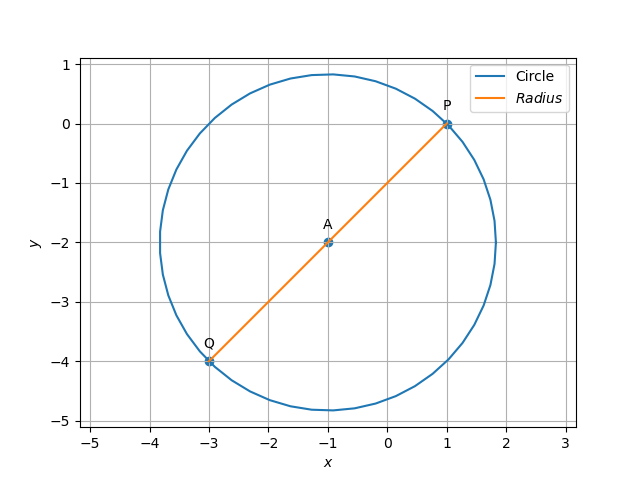
\includegraphics[scale=0.55]{circle.png}
  	\end{center}

\end{multicols}
\end{document}
